\section{PDDL Domain and Problem Classification}

Before running the benchmark, we classified the available PDDL material along two complementary axes. First, we assigned a numerical difficulty score to each domain and instance, so that benchmark results could be interpreted against an explicit complexity estimate. Second, we manually grouped the domains by the main type of reasoning they require.

The initial classification was computed on the 20 source domains stored in the archive of planning domains. The scoring code is located in the framework scripts folderx and the generated CSV/JSON reports are stored in the domain-complexity folder under analysis.

The script used for this step is \texttt{score\_domains\_complexity.py}.

\subsection{Difficulty Classification}

\subsubsection{Instance raw scores}

The complexity of a single problem instance is estimated through a weighted logarithmic combination of four structural metrics. The logarithm reduces the impact of very large feature values, preventing a single component from dominating the score.

The \textbf{raw score} is defined as:
\begin{equation}
    S_{\mathrm{raw}} = 0.45 \cdot \log(1 + A) + 0.20 \cdot \log(1 + G) + 0.20 \cdot \log(1 + N) + 0.15 \cdot T
\end{equation}

where:
\begin{itemize}
    \item \textbf{A (Actions):} estimated number of feasible grounded actions. This is computed by binding action parameters to objects compatible with the static preconditions observed in the initial state.
    \item \textbf{G (Goals):} total number of atomic goal conditions.
    \item \textbf{N (Numeric Score):} composite value representing numeric complexity:
    \begin{equation}
        N = E_{\mathrm{num}} + 2 \cdot P_{\mathrm{num}} + 3 \cdot G_{\mathrm{num}} + M
    \end{equation}
    where $E_{\mathrm{num}}$ is the number of numeric effects, $P_{\mathrm{num}}$ the number of numeric preconditions, $G_{\mathrm{num}}$ the number of numeric goal conditions, and $M$ a binary flag indicating whether the problem defines a metric.
    \item \textbf{T (Topology Score):} spatial or relational complexity extracted from topology-like predicates such as \textit{adj}, \textit{connected}, or similar relations:
    \begin{equation}
        T = \log(1 + \mathrm{Nodes}) + \log(1 + \mathrm{Edges}) + \mathrm{Density}
    \end{equation}
\end{itemize}

The weights are heuristic and can be changed depending on the aspect of complexity that should be emphasized. For example, increasing the weight of $A$ would give more importance to the action branching factor.

The per-instance output is kept as a raw score. These raw scores are used to compare instances inside each domain and to compute domain-level summary statistics such as minimum, median, mean and maximum raw score.

\subsubsection{Domain scores}

The overall difficulty of a domain is not computed as a simple average of its instances. Instead, the framework uses the total amount of instance complexity available for that domain.

The \textbf{Domain Difficulty (0--100)} is computed by:
\begin{enumerate}
    \item summing the $S_{\mathrm{raw}}$ values of all instances belonging to the domain, obtaining a \textit{Total Raw Score};
    \item normalizing this total across all 20 source domains.
\end{enumerate}

With this normalization, the easiest domain receives difficulty 0 and the hardest receives difficulty 100. In the current data, \textit{fo-sailing} is the easiest domain, while \textit{settlersnumeric} is the hardest one.

\subsubsection{Results obtained}

The following heatmaps summarize the numerical classification. The first one shows the normalized domain difficulty score, while the second one compares raw-score statistics across domains.

\begin{figure}[H]
    \centering
    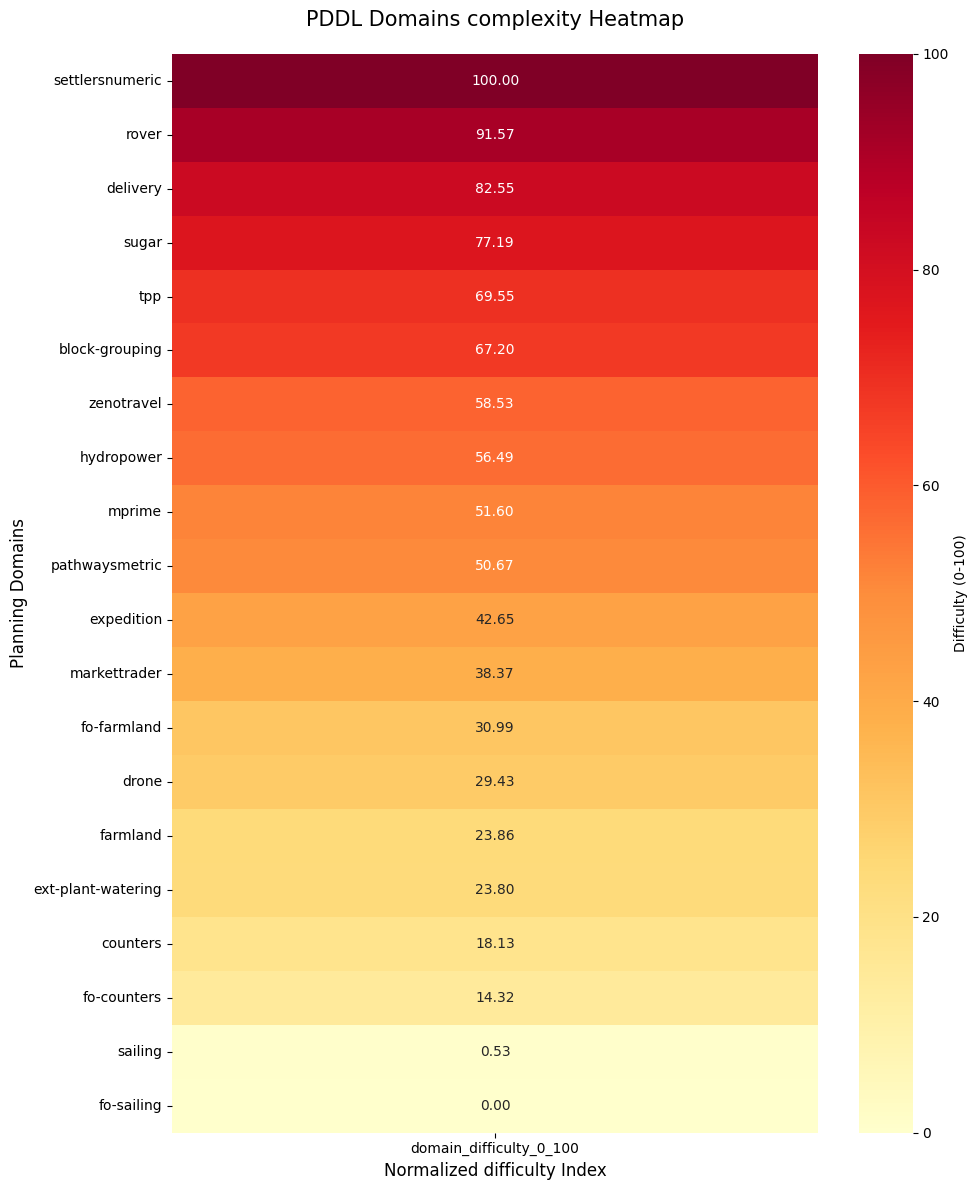
\includegraphics[width=0.6\linewidth]{domaincompl.png}
    \caption{Normalized domain difficulty scores computed from total raw scores.}
    \label{fig:domain-difficulty-heatmap}
\end{figure}

\begin{figure}[H]
    \centering
    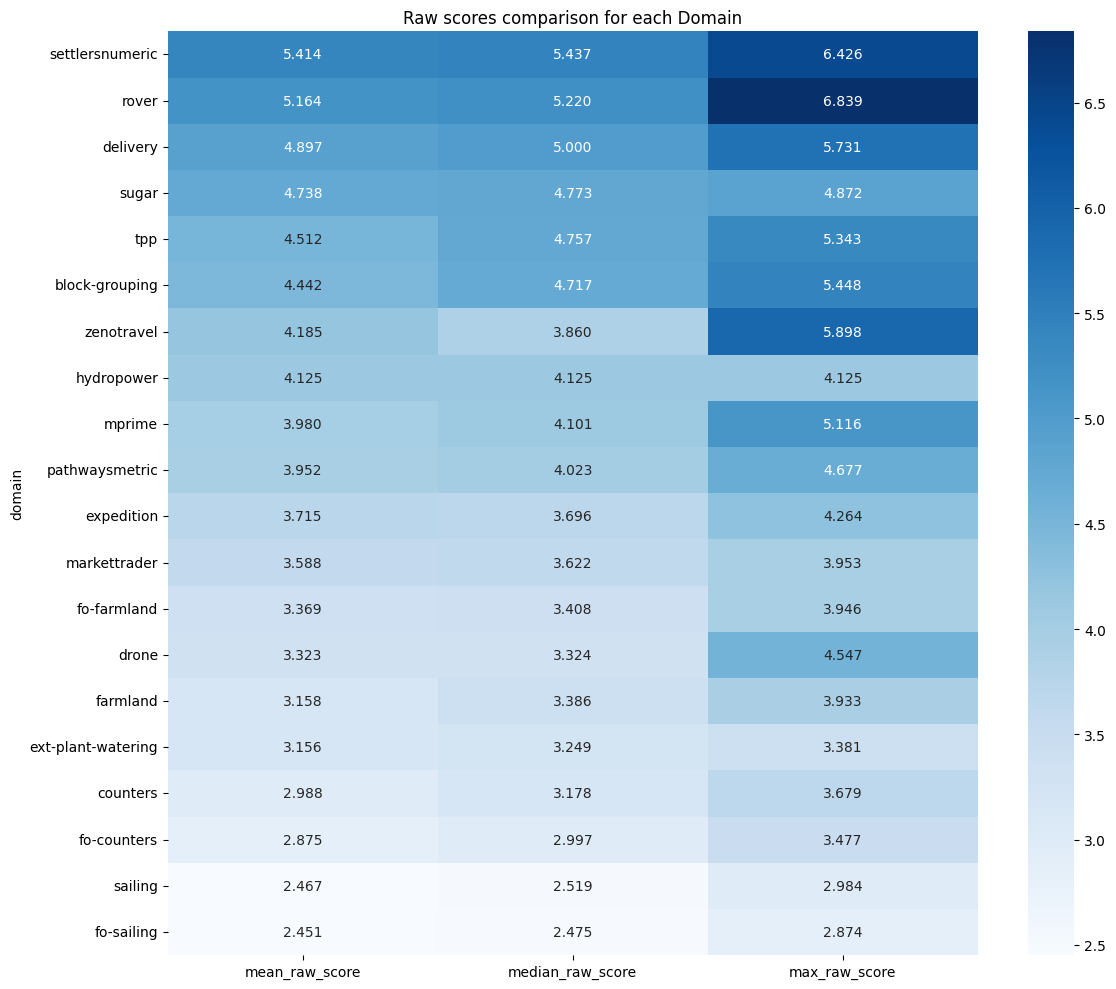
\includegraphics[width=0.6\linewidth]{rawscoreshm.png}
    \caption{Raw-score statistics used to compare the source PDDL domains.}
    \label{fig:raw-score-heatmap}
\end{figure}

\subsection{Reasoning Classification}

In addition to numerical difficulty, we classified each domain according to the main type of reasoning required from the LLM. We used five categories:
\begin{itemize}
    \item \textbf{Spatial:} problems involving objects, agents or resources that must be moved or arranged in a spatial or graph-like environment.
    \item \textbf{Numerical Optimization:} problems requiring management of numeric quantities, costs, resources or objective functions.
    \item \textbf{Temporal Planning:} problems where the solution depends on ordering actions under time-related constraints or temporal relations.
    \item \textbf{Logistics:} problems focused on transportation, delivery, routing or coordination between agents and goods.
    \item \textbf{Logic:} abstract symbolic problems where state transitions represent formal or mathematical transformations rather than physical actions.
\end{itemize}

Table~\ref{tab:reasoning-category-classification} reports the manual classification of the 20 source domains. The rows are ordered from hardest to easiest according to the domain difficulty score described above. When a domain includes multiple reasoning aspects, we assign it to the category that dominates the problem structure. For example, \textit{settlersnumeric} is classified as \textit{Numerical Optimization} because its main challenge is the management of numeric resources and constraints.

\begin{table}[H] \footnotesize
        \centering
        \renewcommand{\arraystretch}{1.25} 
        
        \begin{tabular}{c|c}
            \toprule
            
            \textbf{PDDL Problem} & \textbf{Reasoning Category} \\
            
            \midrule[1pt]
            \addlinespace[0.25cm]
            Settlersnumeric & Numerical Optimization \\
            \midrule
            Rover & Logistic \\
            \midrule
            Delivery & Logistic \\
            \midrule
            Sugar & Numerical Optimization \\
            \midrule
            Tpp & Numerical Optimization \\
            \midrule
            Block-Grouping & Spatial \\
            \midrule
            Zenotravel & Logistic \\
            \midrule
            Hydropower & Temporal Planning \\
            \midrule
            Mprime & Logic \\
            \midrule
            Pathwaysmetric & Numerical Optimization \\
            \midrule
            Expedition & Logistic \\
            \midrule
            Markettrader & Numerical Optimization \\
            \midrule
            Fo-farmland & Numerical Optimization \\
            \midrule
            Drone & Spatial \\
            \midrule
            Farmland & Numerical Optimization \\
            \midrule
            Ext-Plant-Watering & Spatial \\
            \midrule
            Counters & Numerical Optimization \\
            \midrule
            Fo-Counters & Numerical Optimization \\
            \midrule
            Sailing & Spatial \\
            \midrule
            Fo-Sailing & Spatial \\
            
        \end{tabular}
        \vspace{0.2cm}
        \caption{Reasoning Category Classification Tab}
        \label{tab:reasoning-category-classification}
    \end{table}

\subsection{Problems Chosen}

To keep the benchmark compact while still covering different reasoning types, we selected two sets of three problems each. Both sets contain one domain from each of the three categories with enough alternatives for a hard/easy comparison: \textit{Numerical Optimization}, \textit{Spatial}, and \textit{Logistics}. \textit{Temporal Planning} and \textit{Logic} were not selected because the source collection contains only one problem for each of those categories; this would not allow a meaningful difficulty comparison inside the same reasoning type.

The following table shows the domains available in the three selected categories, ordered by decreasing difficulty.

\begin{table}[H] 
    \centering
    \renewcommand{\arraystretch}{1.5}

    \begin{minipage}[t]{0.30\textwidth}
        \centering
        \begin{tabular}[t]{@{}>{\centering\arraybackslash}p{0.9\linewidth}@{}}
            \toprule
            \textbf{Numerical Optimization}\\
            \midrule
            Settlersnumeric\\
            Sugar\\
            Tpp\\
            Pathwaysmetric\\
            Markettrader\\
            Fo-farmland\\
            Farmland\\
            Counters\\
            Fo-Counters\\
            \bottomrule
        \end{tabular}
    \end{minipage}%
    \hfill%
    \begin{minipage}[t]{0.31\textwidth}
        \centering
        \begin{tabular}[t]{@{}>{\centering\arraybackslash}p{0.9\linewidth}@{}}
            \toprule
            \textbf{Spatial}\\
            \midrule
            Block-Grouping\\
            Drone\\
            Ext-Plant-Watering\\
            Sailing\\
            Fo-Sailing\\
            \bottomrule
        \end{tabular}
    \end{minipage}%
    \hfill%
    \begin{minipage}[t]{0.31\textwidth}
        \centering
        \begin{tabular}[t]{@{}>{\centering\arraybackslash}p{0.9\linewidth}@{}}
            \toprule
            \textbf{Logistics}\\
            \midrule
            Rover\\
            Delivery\\
            Zenotravel\\
            Expedition\\
            \bottomrule
        \end{tabular}
    \end{minipage}

    \vspace{0.4cm}
    \caption{Reasoning categories used for the final benchmark selection.}
    \label{tab:selected-reasoning-categories}
\end{table}

The final benchmark uses two sets:
\begin{itemize}
    \item \textbf{Hard Set:} \textit{settlersnumeric}, \textit{block-grouping}, and \textit{rover}.
    \item \textbf{Easy Set:} \textit{fo-counters}, \textit{fo-sailing}, and \textit{expedition}.
\end{itemize}

The hard set contains the hardest domain in each selected reasoning category, while the easy set contains the easiest domain in the same categories. This keeps the reasoning-category distribution fixed and makes the difficulty gap easier to interpret when evaluating LLM outputs.

The selected domains still contain multiple instances. The following heatmap shows that, in general, pfiles increase in raw difficulty as the pfile index grows.

\begin{figure}[H]
    \centering
    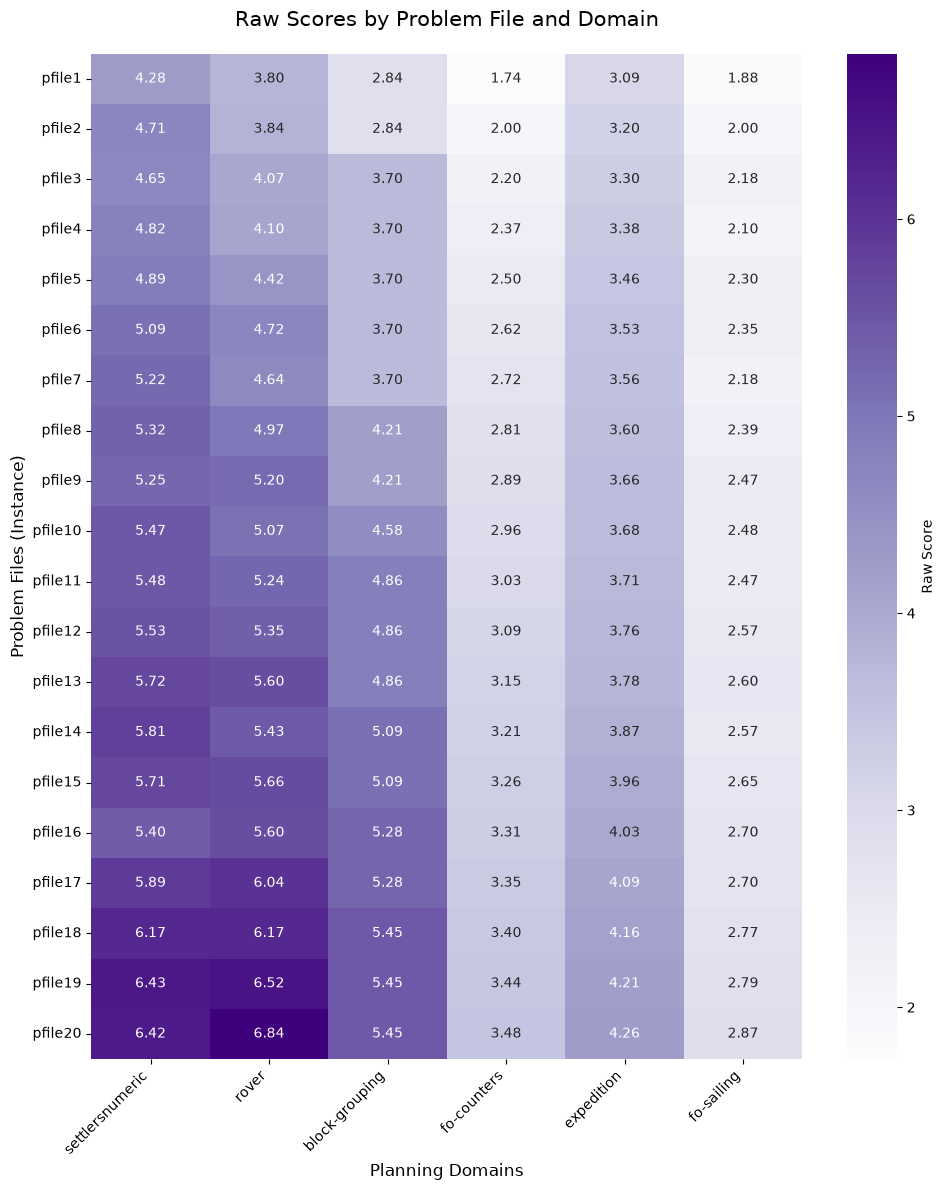
\includegraphics[width=0.55\linewidth]{Instances.png}
\end{figure}

Based on this instance-level trend, we divided the selected pfiles into three difficulty tiers:
\begin{itemize}
    \item \textbf{Easy:} \texttt{pfile1}--\texttt{pfile4};
    \item \textbf{Medium:} \texttt{pfile8}--\texttt{pfile11};
    \item \textbf{Hard:} \texttt{pfile15}--\texttt{pfile18}.
\end{itemize}

Therefore, the final benchmark does not use all available instances from each selected domain. Instead, it uses four instances per difficulty tier, for a total of 12 instances per selected domain.


